\documentclass{article}

\usepackage{microtype}
\usepackage{graphicx}
\usepackage{booktabs}
\usepackage{hyperref}
\newcommand{\theHalgorithm}{\arabic{algorithm}}
\usepackage[preprint]{icml2026}

\usepackage{amsmath}
\usepackage{amssymb}
\usepackage{mathtools}
\usepackage{amsthm}
\usepackage[capitalize,noabbrev]{cleveref}

\theoremstyle{plain}
\newtheorem{theorem}{Theorem}
\newtheorem{proposition}{Proposition}

\newcommand{\FPR}{\mathrm{FPR}}
\newcommand{\E}{\mathbb{E}}
\newcommand{\Bin}{\mathrm{Bin}}
\newcommand{\codelink}{\url{https://github.com/katcinskiy/keylottery}}

\icmltitlerunning{Audit the Deployed Key, Not the Scheme}

\begin{document}

\twocolumn[
  \icmltitle{Audit the Deployed Key, Not the Scheme:\\
    Per-Key False-Positive Control for LLM Text Watermarks}

  \begin{icmlauthorlist}
    \icmlauthor{Alexander Yukhimchuk}{mbzuai}
  \end{icmlauthorlist}
  \icmlaffiliation{mbzuai}{Mohamed bin Zayed University of Artificial Intelligence. ML8502 project proposal}
  \icmlcorrespondingauthor{Alexander Yukhimchuk}{alexander.yukhimchuk@mbzuai.ac.ae}

  \icmlkeywords{watermarking, false positives, LLM, hypothesis testing}
  \vskip 0.3in
]

\printAffiliationsAndNotice{}

\begin{abstract}
The false-positive promise of keyed LLM watermarks is a statement about a \emph{random} key: $\Pr_k[\mathsf{Det}_k(x){=}1]\le\alpha$ for every key-independent human text $x$. A deployed detector uses \emph{one} key, and under it the false-positive rate (FPR) on human text is a lottery. For KGW with a one-token window and Three Bricks scoring, the promise holds on average over 1000 keys, but at $\alpha=10^{-3}$ the 1-in-100 key flags 2.7--3.0$\times$ the promised rate on English text, 5.7$\times$ on code and 9.9$\times$ on Russian (ideal keys: 1.7$\times$), and the worst key 65$\times$. We propose to audit the deployed key rather than the scheme: predict a candidate key's FPR from public text, deploy only keys that pass, attack the audit adaptively, and map how the lottery depends on the window size and the scheme (SynthID-Text). In a preliminary experiment, keeping the 20\% least-biased keys reaches the ideal worst-domain level (${\le}1.84\times$) on unseen text, at an estimated 3 points of detection rate against about 10 for tightening the threshold.
\end{abstract}

\section{Problem}
\label{sec:problem}

\textbf{The promise.} KGW-style watermarks \citep{kirchenbauer2023watermark} colour each token green or red by a pseudo-random function of a secret key $k$ and a \emph{window} of the previous $h$ tokens, with a fraction $\gamma=0.25$ green, and flag a text with too many green tokens. The provider picks the false-positive rate $\alpha$ it promises. With Three Bricks scoring \citep{fernandez2023three}, each distinct (window, token) pair is counted once and tested exactly: a 200-token English text has $T\approx180$ distinct pairs, its green count is $\Bin(180,\tfrac14)$ with mean 45 under a random key, and at $\alpha=10^{-3}$ it is flagged at ${\ge}65$ greens, the smallest count a random key reaches with probability ${\le}\alpha$ ($z\approx3.4$; exact level $0.6\alpha$). The guarantee is over the key draw, for each fixed human text \citep{zhao2025sok}.

\textbf{What fails.} A provider draws the key once. Counting each pair once removes repeats \emph{inside} a text, not \emph{across} texts: under the deployed key a frequent pair such as ``. The'' (in 28\% of news texts) has the same colour in every document, so a key that happens to colour several frequent pairs green shifts all texts of a domain at once. A user faces $\FPR(k)=\Pr_{x\sim D}[\mathsf{Det}_k(x)=1]$ for the deployed $k$; the promise only gives $\E_k\FPR(k)\le\alpha$.

\textbf{Measured.} Window \mbox{$h=1$} (the previous token only; transformers' default \texttt{lefthash}), OPT tokenizer \citep{zhang2022opt}, 200 scored tokens, five human-text domains (C4 news, English Wikipedia, Wikipedia ``List of'' pages, Python files, Russian Wikipedia), 1000 fresh random keys, 6000 unseen texts per domain (\cref{fig:lottery}); the watermark bias $\delta$ does not enter the FPR. At $\alpha=10^{-3}$ the FPR averaged over keys is $0.61$--$0.78\,\alpha$. But the 1-in-100 key (99th percentile over keys, roughly the 10th worst of 1000) flags 2.7$\times$ (news), 3.0$\times$ (English Wikipedia), 2.7$\times$ (lists), 5.7$\times$ (code; 95\% CI 3.3--8.8) and 9.9$\times$ (Russian; 6.0--34), against 1.67$\times$ for ideal keys at this sample size. The worst key flags 65$\times$ (Russian); on code the worst, 64.7$\times$, is one key times one licence-header cluster. Per-key flag counts are overdispersed everywhere (index of dispersion 10--46 at $\alpha=10^{-2}$, 825 on Russian; ideal: 1). An idealised hash gives the same picture, and our code reproduces transformers' detector exactly. Caveats: over a third of our unseen Russian texts are templated village stubs, and OPT splits Cyrillic into byte-level pieces (re-tokenized with Qwen2.5 at equal $T{=}55$: ${\approx}2\times$ vs.\ $4.2\times$ under OPT). We make no claim about any provider's key.

\textbf{For whom, why now.} Deployed detectors run with one fixed key: SynthID-Text marks Gemini responses \citep{dathathri2024scalable}; Anthropic marks Claude with a version of it and offers detection to eligible organisations, educational ones included \citep{anthropic2026watermark}; the EU AI Act's marking duty (Art.~50(2)) applies from 2 August 2026. A student whose code is checked faces the FPR of the deployed key: screening $10^5$ submissions at $\alpha=10^{-3}$ promises 100 false accusations, but under the 1-in-100 key makes about 570. If every provider watermarks with its own key, a human text faces many keys, and the unlucky ones dominate. The window size decides which texts are exposed: with one token every frequent pair matters; with SynthID's four tokens only repeated sequences do (templates, boilerplate, set phrases). For a 4-token window a formula-only forecast (\cref{prop:var} with 4-token statistics, $\alpha=10^{-2}$) predicts the ideal level on English prose but ${\approx}3\times$ on code, which our first experiment tests.

\begin{figure}[t]
  \centering
  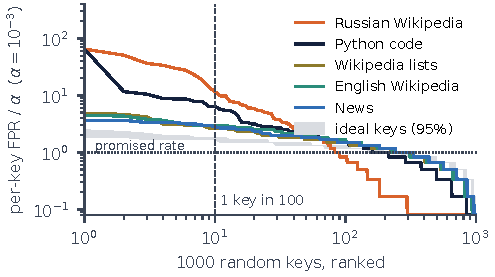
\includegraphics[width=\columnwidth]{figs/fig_lottery.pdf}
  \vspace{-6mm}
  \caption{Per-key FPR of Three Bricks scoring ($h=1$) for 1000 fresh keys, ranked from worst, on 6000 unseen human texts per domain, $\alpha=10^{-3}$. Dashed: the 1-in-100 key. Gray: 95\% band of identical ideal keys.}
  \label{fig:lottery}
  \vspace{-3mm}
\end{figure}

\section{Success metrics}
\label{sec:metrics}

Two axes, false accusations and detection (\cref{fig:pareto}), plus the success of our own attack; each is reported per window size $h\in\{0,1,2,3,4,8\}$ and scheme (\cref{sec:idea}). All metrics and the thresholds of \cref{sec:falsification} are fixed before the experiments. Code: \codelink.

\textbf{M1. False accusations.} FPR$/\alpha$ of the 1-in-100 key on unseen human text, per domain and worst of five, at $\alpha\in\{10^{-2},10^{-3}\}$, with order-statistic 95\% intervals over keys. Target: the ideal-key level $L(n,\alpha)$, the 99th percentile of $\Bin(n,\alpha_D)/(n\alpha)$ with $\alpha_D$ the exact test's realised level (1.67 per domain and 1.83 worst of five at $n=6000$, $\alpha=10^{-3}$; 2.0 at the nominal $\alpha$). Below $10^{-3}$ M1 is reported through the audit's prediction, a lower bound on the tail (a conditional mean), checked against flags pooled over keys (F2).

\textbf{M2. Detection.} TPR at the promised $\alpha$, clean and with 20\% of tokens replaced, 30 keys per method, on news (OPT-1.3B), code and Russian (Qwen2.5-1.5B) prompts, at $\delta\in\{1,2\}$. At $\delta=2$ tightening tenfold costs only 0.2 points (2 under swaps), so the trade-off concerns weak, short or edited marks.

\textbf{M3. Framing rate} under the attacks of \cref{sec:threat}: the share of the adversary's 100 texts flagged at $\alpha=10^{-3}$ after $B\in\{0,10^3,10^4\}$ queries, 30 audited vs.\ 30 random keys; edited texts must keep their perplexity under Llama-3.1-8B within the domain's human 95th percentile.

\section{Related work and baselines}
\label{sec:related}

\textbf{Schemes and false positives.} KGW \citep{kirchenbauer2023watermark}, its fixed-list case $h=0$ \citep{zhao2024provable} and SynthID-Text \citep{dathathri2024scalable} evaluate keyed functions of (window, token), so the lottery can arise in each; position-keyed sampling \citep{kuditipudi2024robust} is out of scope. \citet{kirchenbauer2024reliability} score repeated pairs once; \citet{fernandez2023three} add exact tests and validate the FPR with texts pooled over 10 keys. Key dependence of the null has been noted: \citet{gloaguen2026diffusion} report FPR at $\alpha=1\%$ over 100 keys on news (worst key 17\% for $h=0$, 1.7\% for $h=1$) and conclude that hashing a window suffices in practice; \citet{fernandez2025posthoc} pick their key among 50 by a uniformity test on 100 texts; \citet{li2026tiwm} is concurrent. None measures the tail at operational $\alpha$, explains or predicts it, or attacks the selection. \citet{gloaguen2025spoofing} detect spoofing through the coupling of colours and n-gram frequency that our audit uses. \textbf{Attacks:} watermark stealing \citep{jovanovic2024stealing}, framing human text under OPT with $h=1$ \citep{sadasivan2025reliably}, adaptive removal \citep{diaa2025optimizing}, key pools against forgery \citep{aremu2026randomized}.

\textbf{Baselines on our metrics} (\cref{tab:baselines}, \cref{fig:pareto}), on the same keys and texts. All-token KGW breaks the promise; Three Bricks keeps detection, but its 1-in-100 key is 9.9$\times$. \emph{Masking frequent pairs} (our first fix, which failed: not scoring pairs in over 1\% of public texts) cuts the key-to-key variance of the mean $z$ 17--27$\times$ (3.6$\times$ on Russian) but leaves the lottery. \emph{Tightening} to $\alpha/10$ (testing at $\alpha/10$, promising $\alpha$) reaches 0.5$\times$ for 18 TPR points, yet its worst key is still 20.5$\times$ on code; the minimal sufficient tightening costs about 10 points by interpolation, which we will measure. A \emph{key pool} \citep{aremu2026randomized}, built against forgery, marks each response with one of $r$ keys and attributes a text if exactly one key fires at the Šidák level ${\approx}\alpha/r$; it averages its keys' FPRs to 3.0$\times$ at $r=10$ (5.2$\times$ at the paper's $r=4$) for the TPR of tightening $r$-fold, and auditing each pool key composes with it. \emph{Per-key calibration} ($z$-standardising each key on reference text) fixes the mean in-domain but not across domains (calibrated on news: 5.0$\times$ on code, 8.0$\times$ on Russian at the 1-in-20 key); its strongest form, a per-key split-conformal threshold \citep{xie2025classroom}, will be added.

\begin{table}[t]
  \caption{Baselines at the promised $\alpha=10^{-3}$, $h=1$. FPR: 1000 fresh keys $\times$ 6000 unseen texts per domain, worst domain. TPR: OPT-1.3B, $\delta=1$, the same 10 random keys $\times$ 400 prompts. $^a$Three Bricks TPR minus the estimated cost (3.0/3.5 points); measured on 10 audited keys: 0.84/0.35. $^b$1-in-100 of 20{,}000 pools; one licence-header key in 1\% of pools makes this 3.0$\times$ or 21$\times$ by draw. $^c$TPR at ${\approx}\alpha/10$.}
  \label{tab:baselines}
  \vskip 0.05in
  \centering
  \small
  \begin{tabular}{lrrr}
    \toprule
    Method & 1-in-100 key & TPR & 20\% swap \\
    \midrule
    KGW, all tokens & 452$\times$ & 0.83 & 0.38 \\
    Three Bricks & 9.9$\times$ & 0.84 & 0.37 \\
    Masking frequent pairs & 5.2$\times$ & 0.82 & 0.31 \\
    Tighten to $\alpha/10$ & 0.5$\times$ & 0.66 & 0.18 \\
    Key pool, $r=10$\,$^b$ & 3.0$\times$ & 0.66$^c$ & 0.18$^c$ \\
    \midrule
    Audited keys (prelim.) & 1.8$\times$ & 0.81$^a$ & 0.33$^a$ \\
    Ideal keys (worst of 5) & 1.8$\times$ & -- & -- \\
    \bottomrule
  \end{tabular}
  \vspace{-3mm}
\end{table}

\section{Idea: audit the deployed key}
\label{sec:idea}

Four parts: map the lottery over window size and scheme; an \emph{audit} that predicts a candidate key's FPR from public text; a \emph{defence} that deploys only keys that pass; and our own adaptive \emph{attack} on the audit (\cref{sec:threat}), since the audit rule is public.

\textbf{Scope: window size and scheme.} We first rerun the null for KGW at $h\in\{0,1,2,3,4,8\}$ (LeftHash and SelfHash), for SynthID-Text at its deployed window of four tokens with its within-document masking of repeated windows, and for Unigram ($h=0$). The theory below holds for any $h$: only the set of shared (window, token) pairs changes.

\textbf{Audit: why keys differ (done).} For $n$ texts let \mbox{$A_{xu}=1$} if pair $u$ occurs in text $x$, $T_x=\sum_uA_{xu}$, $z_x=(G_x-\gamma T_x)/\sqrt{\gamma(1-\gamma)T_x}$ with $G_x$ the green count, $\bar z=\frac1n\sum_xz_x$ and $a_u=\frac1n\sum_xA_{xu}/\sqrt{T_x}$.
\begin{proposition}
\label{prop:var}
If each window's green list is a uniformly random set of $\gamma V$ of the $V$ tokens, independently across windows, then $\E_k\bar z=0$ and $\mathrm{Var}_k\bar z=\big(V\sum_ua_u^2-\sum_cS_c^2\big)/(V-1)$, where $S_c$ sums $a_u$ over pairs $u=(c,w)$ with window $c$; for i.i.d.\ Bernoulli$(\gamma)$ colours $\mathrm{Var}_k\bar z=\sum_ua_u^2$.
\end{proposition}
A pair in a fraction $p_u$ of texts contributes about $p_u^2/T$, so a few frequent pairs carry the variance. The formula matches measurement in 203 of 210 cells (7.1 deviations expected by chance) over four orders of magnitude, for $h\in\{0,1\}$ and two hash functions.

\textbf{Audit: predicting a key's FPR.} The audit reads the key's colours $g_F(k)$ on a set $F$ of pairs frequent in public reference text of each domain. For a text $x$ let $S^F_x(k)$ count its green pairs in $F$, $T^R_x$ its pairs outside $F$, and $c_\alpha(T)$ be the exact-test threshold.
\begin{proposition}
\label{prop:pred}
If colours outside $F$ are i.i.d.\ Bernoulli$(\gamma)$, independent of $g_F(k)$, and $D$ does not depend on $k$, then $\E[\FPR(k)\,|\,g_F(k)]=\hat F(k)$, where $\hat F(k):=\E_{x\sim D}\Pr\big(\Bin(T^R_x,\gamma)\ge c_\alpha(T_x)-S^F_x(k)\big)$.
\end{proposition}
This follows from Fubini, since the pairs of a text are distinct; it needs no independence between texts and holds at any $\alpha$ (fixed-size green lists add an $O(|F_c|/V)$ error; $F$ and the average over $x$ use disjoint halves of the reference text). With $F$ the pairs shared within the evaluated corpus it is exact by construction, and $\hat F$ matches counted flags ($|z|\le2.05$ in 60/60 cells), a check of code and model. With $F$ from public text only the transfer of a key's mean bias is tested so far (correlation 0.82--0.996 across keys); testing $\hat F$ out of sample is the first deliverable. A concentration bound around $\hat F$ \citep{freedman1975tail} is a stretch goal: $n$ texts cannot certify an FPR below $-\ln(0.05)/n\approx3/n$ without assumptions on $D$, so below that the audit predicts relative to a fixed public corpus.

\textbf{Defend.} Deploy only keys with $\hat F_d(k)\le\alpha$ in every covered domain $d$ (fixed now; under \cref{prop:pred}, $\E[\FPR_d\mid\text{deployed}]\le\alpha$); text that a public domain classifier does not assign to a covered domain is tested at $\alpha/10$. Generator, detector and test are unchanged; rejecting a fraction $1-q$ of keys costs $\log_2(1/q)$ bits of key entropy. A template filter for clusters no key passes changes the test and is reported as a variant.
\emph{Preliminary experiment.} A simpler rule keeps the 20\% least-biased of 1000 fresh keys, a key's \emph{bias} being its largest standardised mean $z$ over the five reference sets (how strongly it colours their frequent pairs green). On unseen texts the 1-in-100 key drops from 2.7--9.9$\times$ to ${\le}1.84\times$ at $\alpha=10^{-3}$ in all five domains, the ideal worst-of-five level (point estimate over 200 kept keys; worst kept key 7.8$\times$ vs.\ 65$\times$). Nine of ten (domain, $\alpha$) cells pass the nominal floor (eight against 1.67$\times$); the miss is code at $10^{-2}$ (1.9$\times$ vs.\ 1.3$\times$, caused by licence headers), and on an older unseen set code is 2.7$\times$. A direct detection test (10 audited vs.\ 10 random keys, at $\alpha=10^{-4}$) gives $-0.4$ points (95\% CI $[-5.1,4.2]$), too noisy to resolve the cost. A regression explains the cost: a key that colours frequent pairs green both flags more humans and catches more model text (TPR correlates 0.93 with its bias on news), which puts the cost at about 3 points. One hypothesis failed: kept keys are conservative (mean FPR 0.37--0.48$\alpha$, 0.01$\alpha$ on Russian) and still differ (dispersion 3--105), so the selection removes the tail, not the lottery.

\textbf{Why Pareto-optimal.} Tightening raises the threshold for every key to pay for the worst one, and a pool pays the same through its Šidák level; the audit removes only the bad keys and leaves the test untouched, so its cost is only the link between a key's bias and its power: about 3 points against about 10 (\cref{fig:pareto}). Against masking the case is open. Masking reaches the ideal level in 8 of 10 cells (failing only on templated Russian) for 1.9 points on the same random keys; with the same bias adjustment it costs 4.3 points clean and 8.7 under swaps (audit: 3.0, 3.5), and it scores only 78 of 138 pairs on code and 10 of 139 on Russian. On the older unseen set, however, its worst cell (2.0$\times$) beats the audited keys' (2.7$\times$). F3 decides.

\begin{figure}[t]
  \centering
  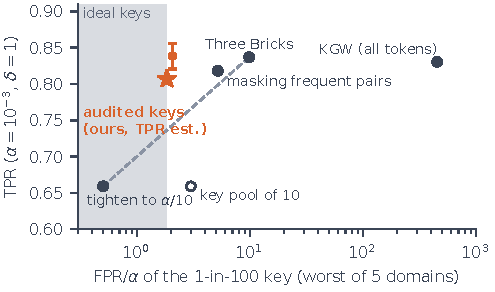
\includegraphics[width=\columnwidth]{figs/fig_pareto.pdf}
  \vspace{-6mm}
  \caption{Detection vs.\ the FPR of the 1-in-100 key (\cref{tab:baselines}). Dashed: tightening, interpolated. Star: audited keys, random-key TPR minus the estimated cost; bar: measured on 10 audited keys, 95\% CI. The 10 random keys happen to be low-bias, so all points sit a few TPR points low together.}
  \label{fig:pareto}
  \vspace{-3mm}
\end{figure}

\section{Threat model}
\label{sec:threat}

\textbf{Defender:} a provider with one secret key (or a pool), public reference corpora, a public domain classifier and the audit. \textbf{Adversary:} wants to \emph{frame a human}, i.e.\ have a fluent human-quality text flagged under the deployed key. Following Kerckhoffs, it knows the scheme, the audit rule and the corpora, but not the key; it can query the watermarked model, not the detector. Removing the mark is out of scope beyond M2's 20\% swaps (audited keys mark more weakly, as TPR tracks bias). Three routes:
(A1) \emph{Coverage, no queries:} human text the audit did not see, a held-out domain or the most templated slice of an audited one. Both beat an audit-only defence in our experiment (held-out code and Russian: 4.3$\times$ and 22.5$\times$ at $\alpha=10^{-2}$, as for random keys; worst kept key 7.8$\times$, all licence headers), hence $\alpha/10$ for unclassified text and the template variant; the defence holds if kept keys stay within $L(n,\alpha)$ on every slice the classifier accepts.
(A2) \emph{Stolen green pairs:} estimate them by stealing \citep{jovanovic2024stealing,sadasivan2025reliably}, then select human texts, or edit at most 20\% of a victim's tokens, to be dense in them.
(A3) \emph{Adaptive to the audit:} with no queries, sample $10^4$ keys that pass the public audit and select or edit human texts to maximise their mean flag rate over these keys, exploiting any structure the audit imposes (frequent pairs red, so rare pairs carry the signal); with queries, add A2's stolen pairs. Texts built from queries depend on the key, so no per-key guarantee covers them; M3 measures them.
\textbf{Ethics.} Attacks target only our own keys on local open models; no deployed detector is queried and no provider's key is sought. If the lottery holds for the open SynthID-Text or transformers defaults, we notify the maintainers before publication.

\section{Falsification and risks}
\label{sec:falsification}

On fresh keys and unseen texts the idea is falsified if: (F1) on 5000 fresh keys, in more than one of the ten (domain, $\alpha$) cells, more deployed keys exceed the 99th percentile of $\Bin(n,\alpha_D)$ than ideal keys allow (one-sided binomial test against $\Bin(K,0.01)$, $p<0.05$); (F2) with $F$ from public text only, the Spearman correlation over keys between $\hat F$ and counted FPR is below 0.5 at $\alpha=10^{-2}$, or pooled flags differ from $\sum_kn\hat F(k)$ by $|z|\ge3$ (s.e.\ from per-key residuals) at any $\alpha\in\{10^{-2},\dots,10^{-5}\}$; (F3) some baseline (measured tightening, per-key conformal threshold, key pool, masking), at its weakest setting that passes F1, has higher TPR in some domain, the 95\% CI of the bias-adjusted difference over 30 keys per arm excluding zero; (F4) at some budget $B$ more A1--A3 texts are flagged under audited than under random keys (one-sided permutation test over keys, $p<0.05$); (F5) at SynthID's window and at $h=4$, the index of dispersion of per-key flags at $\alpha=10^{-2}$ is ${\le}1.5$ in every domain once files sharing a 32-token span are removed: then the lottery is a short-window and template effect, and all claims are restricted to those.
\textbf{Risks.} (i) Window size (F5). (ii) Russian under OPT is partly a tokenizer and sample artefact. (iii) The detection cost is a model estimate and vanishes for strong marks. (iv) The audit may just select conservative keys; matched-M1 comparisons address this. Our experiments already refuted three of our own pre-registered hypotheses (masking and key selection do not remove the lottery; cross-domain calibration fails less than predicted).

\section{Compute and plan}
\label{sec:compute}

All jobs run under Slurm on the course cluster (Titan). The preliminary experiments took about 2.5 hours: the null on 1000 keys $\times$ 15k texts per domain takes 28\,min on 32 CPU cores; 8000 watermarked OPT-1.3B texts take 21\,min on 4 of 10 shards of an RTX PRO 6000. Plan: (1, late October) nulls over window size and scheme (KGW LeftHash/SelfHash with an idealised hash, SynthID-Text via its transformers implementation, Unigram), the Qwen2.5 tokenizer and a 5000-key rerun for F1, ${\approx}100$ CPU-hours; measured tightening, conformal and pool baselines, TPR and perplexity on 30 keys per arm (OPT-1.3B news, Qwen2.5-1.5B code and Russian), ${\approx}4$ GPU-hours; (2, November) out-of-sample test of $\hat F$, template filter, domain classifier, and A1--A3 on 30+30 keys, stealing from next-token samples on cached OPT-1.3B logits of $10^4$ human prefixes (a key changes only the sampling), ${\approx}1$ GPU-hour; (3, December) report and talk. Budget: about 150 CPU-hours and 10 GPU-hours.

\bibliography{refs}
\bibliographystyle{icml2026}

\end{document}
